\vspace{-1mm}
\section[Envisioned Future for Robotic Surgery at Aalborg University Hospital]{Envisioned\,Future\,for\,Robotic\,Surgery\,at\,Aalborg\,University\,Hospital}\label{sec:aau_doc}

\vspace{-2mm}
At Aalborg University Hospital robotisized \gls{mis} has been implemented since 2008, and now count two da Vinci surgical robots employed at the urology and gynaecological wards, each performing 230 surgeries a year. %(og en i dyrelaboratoriet til at øve på)
The authors were granted access to attend a prostatectomy at the hospital, during which robot assistant nurse Jane Petersson explicated the spectacle on the monitors revealing the process of gaining access to the cancerous prostate, cleaving way through tissue involving exposure of veins and nerves that must not be cut during the surgery. A view from the surgery is seen in \autoref{fig:surgery} showing the da Vinci robot reaching into the patient's abdomen.
\begin{figure}[htbp]
	\centering
	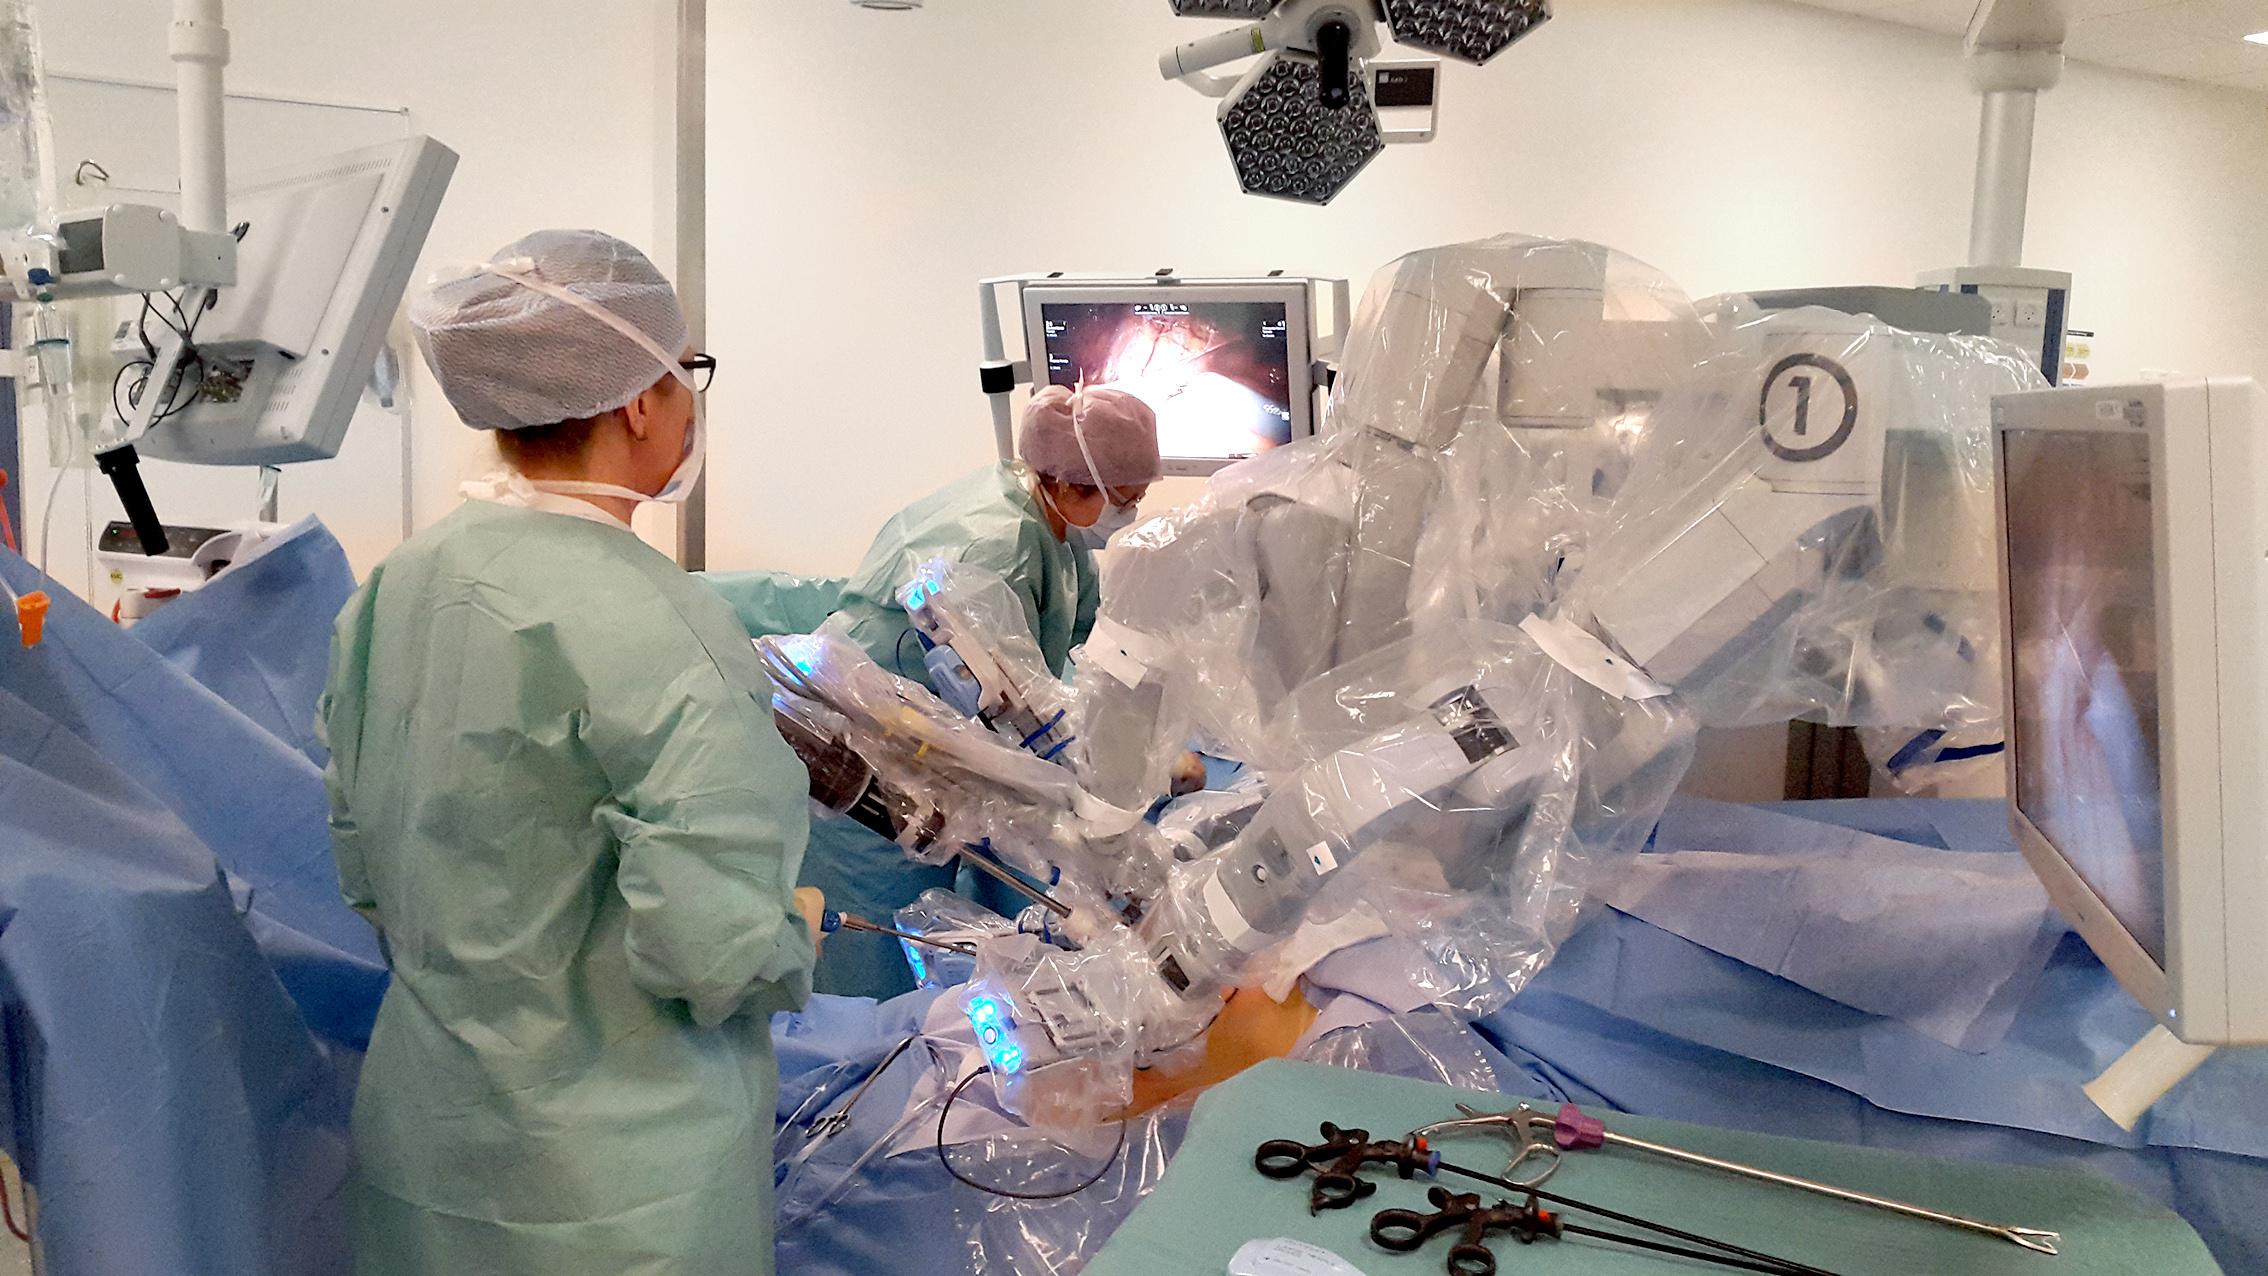
\includegraphics[width=0.88\textwidth]{20150526_103311.jpg}
	\caption{Prostatectomy at Aalborg University Hospital conducted by surgeon Grazvydas Tuckus with the da Vinci Xi robot. The robot arms are wrapped in sterile bags.}
	\label{fig:surgery}
\end{figure}

\phantom{.}

\vspace{-12mm}
Johan Poulsen, chief surgeon at the urology ward and manager of the Center for Minimally Invasive Surgery at Aalborg Univeristy Hospital, concurs with the stance that robotic laparoscopy provides the surgeon with greater dexterity, stability and precision due to the design of the robot tools, the tremor filtering, micro-movement down-scaling %of approx 10-15 times
and 3D visual overview of the surgical site.  %a 2D camera used in manual laparoscopy.
It also allows the surgeon a much better work posture than manual laparoscopic surgery and he argues that it is easier to learn operating the robot than manual laparoscopic tools, %not least for the suturing technique, 
and with the generations now entering the job market mastering  robotic technologies for surgery will come naturally.

At present the da Vinci robot is routinely used in Denmark in procedures within gastroenterology, gynaecology and urology. Dr. Poulsen, who is one of the nationally leading experts within robotic surgery, argues that the next few years will also see robotics applied in surgery of the alimentary tract as well as in otorhinolaryngological, lung and heart surgery, in pace with the purchase and maintenance price of surgical robots going down.

According to Dr. Poulsen one of the greatest challenges in operating on a beating heart is the concluding part of the operation suturing the operation site, as the moving tissue is easily pinched or tugged. 
In order for the advantages of robotisized heart surgery to compensate for the drawbacks of manual bypass operations, it is paramount to have a very exact model of the heart movement. 
As the heart movement is not a beat as such but rather an expansion and contraction movement propagating from one end of the heart to the other, even a highly complex model will need correction from position measurements of the surface of the heart. 
He sees it as a viable possibility to mount sensors of up to two by two centimetres by sowing them to the surface of the heart and having a tracking system such as e.g. the Vicon system (Vicon is an indoor  tracking system similar to the outdoor GPS) being part of the range of surgical instruments in order to get extremely exact position data for the motion-compensated surgical robot.


Dr. Johan Poulsen suggests a surface mounted on a cylinder, which can be controlled to periodically move up and down, as a first step in testing a surgical robot in following the movement of a surface.





%så ser han den også blive brugt indenfor mave/tarm, øre/næse/hals, mikrokirurgi, hjerte, lunge, og mener bestemt det er fremtiden



%Forhindringer
%
%The cost price of 15 million DKK is too high (Johan Poulsen)
%
%fremtid: folk skal kunne se fordelen ved at bruge den i forskellige typer af operationer, men det er meget prisen der sætter begrænsningen, Intuitive holder prisen utroligt højt oppe, indkøbspris ca 25 mio kr, plus årlig service på 2.5 mio kr, plus 1600-1500 kr pr instrument som kun kan bruges 10 gange. Johan Poulsen vurderer at det skal ned i 1/5 pris for at det kommer ind på mange andre områder, 
%

\vspace{-2mm}
\section{Establishment of da Vinci at Aalborg University}\label{sec:technical_overview}
%A surgery consists of a series of subtasks, some suited for robotized autonomous execution. Prior work in motion planning and control of subtasks for surgical robots include knot tying, suturing and more advanced statistical learning of subtasks from recording surgeon motions \citep{bib:raven_debride,bib:raven_observ}.

\vspace{-2mm}
The configuration at the Control and Automation laboratory at Aalborg University is based on a first generation da Vinci robot, where the patient manipulator is detached from its surgeon controller console and modified to be controllable by automated processes. %The setup is physically located at  Aalborg University.
As seen in \autoref{fig:master-slave_surgery} the da Vinci patient manipulator constitutes four "arms". In this thesis controllers are developed for one of these arms, 
%Before a technical overview of the system is given, 
an overview of the terminology used for the robot  outlined in \autoref{fig:naming_convention},
\begin{figure}[htbp]
\centering
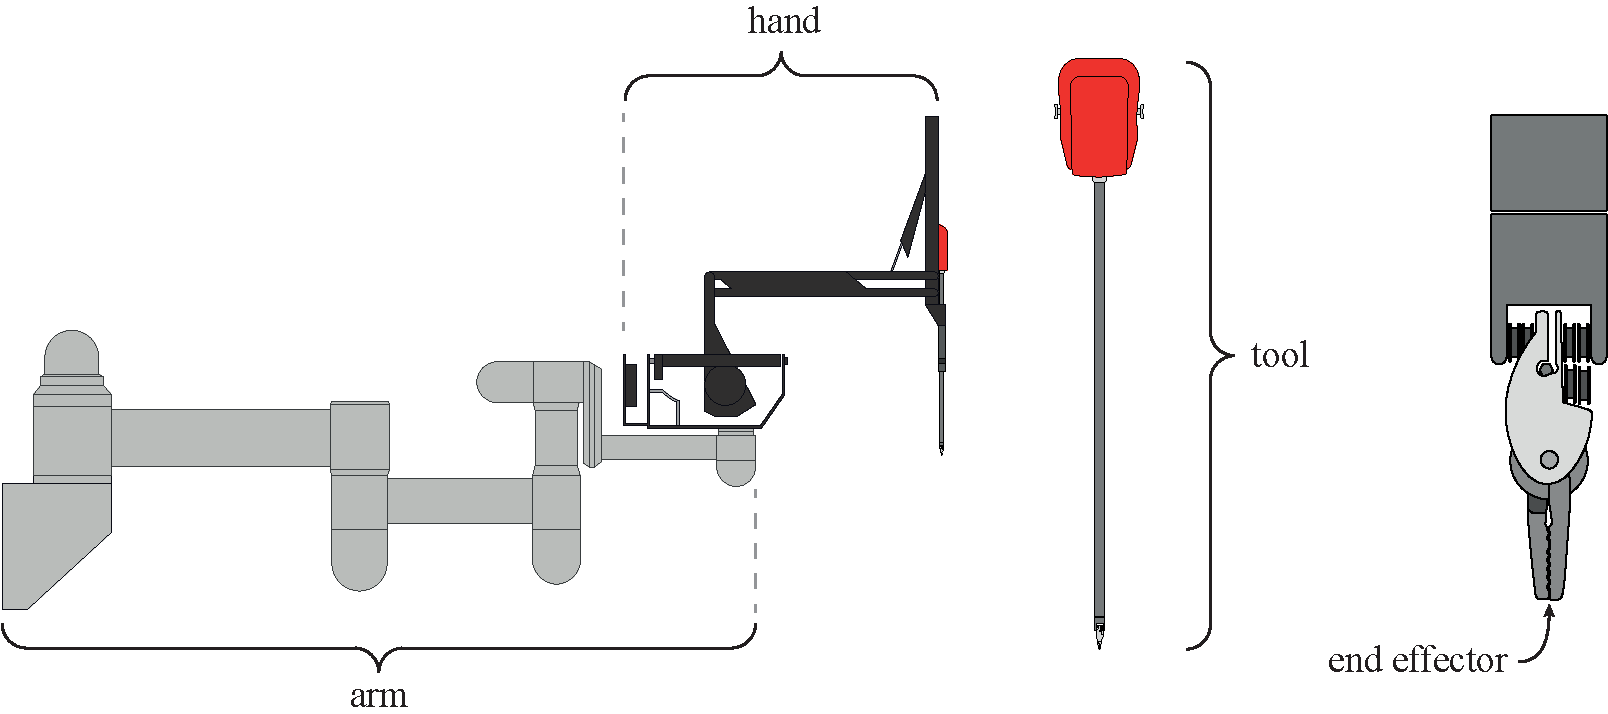
\includegraphics[width=0.8\textwidth]{naming_convention.pdf}
\caption{Naming convention used for the da Vinci robot.}
\label{fig:naming_convention}
\end{figure}
depicting the distinction of the robotic parts each comprising a number of links. 
The far left part is termed the "arm" and its joints are fixed by electromagnets and hence uncontrollable, but can be manually released for positioning. 
The center left part labelled the "hand" consists of the controllable dynamic joints, including the "tool", located center right, which is a replaceable instrument worth 10.000\,kr only licensed to be used for 10 operations. The outermost point of the instrument is labelled the "end-effector" and it is  this which should follow a reference point in the developed controllers.

%
%\subsection{Technical Overview of the Robotic Surgery System}
%A simplified overview of the robot controller setup is provided in \autoref{fig:overview}. 
%
The technical overview presented in \autoref{fig:overview} is structured in descending abstraction layers with the highest in the top (i.e. the \gls{ros} - an open source software framework for robots \citep{bib:ros}, see \autoref{app:ros} for further details), which establishes a wireless TCP/IP communication channel receiving all positions from the robot as feedback and produces position control signals to the NI (National Instruments) single board \glspl{rio} which handle all input/output communication with the user. The NI single board \glspl{rio} consist of a primary and a secondary board. The reason for having two \gls{rio} boards is solely the lack of input/outputs on one board.

\begin{figure}[H]
	\hspace*{-5mm}
	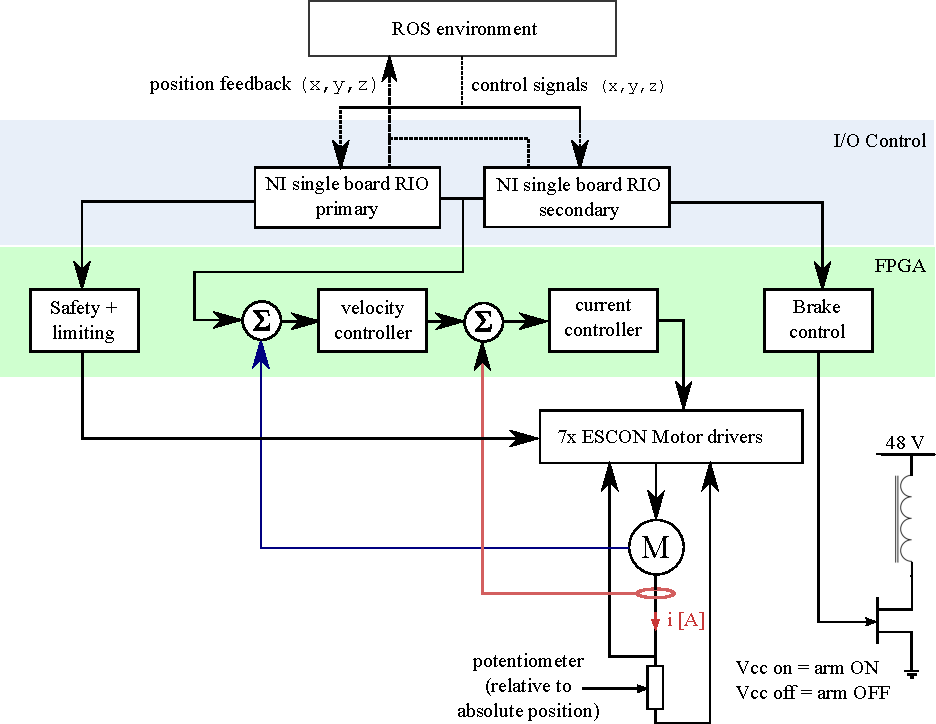
\includegraphics[width=1.09\textwidth]{overview.pdf}	
	\caption{Overview of the custom made hardware and controllers for the 1st generation da Vinci surgical robot located at Aalborg University's department of Control and Automation.}
	\label{fig:overview}
\end{figure}

The \gls{rio} boards direct the control signals to a cascaded controller taking in a position reference from the user and delivering a current control signal to the ESCON motor driver. The velocity and current controllers are implemented in \gls{fpga} based hardware to ensure sufficient controller speed relative to the system \citep{bib:robot_paper}. The ESCON motor driver manages advanced processing and essentially delivers an appropriate PWM signal for the actuators (seven Maxon motors) which represent the lowest abstraction layer, located at the bottom of the figure.

The NI single board \glspl{rio} concurrently handle most safety precautions and enabling/disabling movement of the arm itself (see \autoref{app:links_joints_3d} and \ref{app:kinematic_model_robot} for an overview of the arm and its kinematics, respectively) through solenoids.
%
In order to prevent potential violation of physical joint constraints, stricter constraints on each joint position are set in the low-level motor controllers, that disable the controller if exceeded.

An introduction to the da Vinci system has at this point be given. Thus the contribution of this project will be outlined in the upcoming subsection.


\subsection{Overview of Thesis Contribution to the AAU da Vinci System}\label{sec:project_overview}
The focus of this thesis is the highest abstraction layer as seen in the top of \autoref{fig:overview}, i.e. the ROS environment. The purpose of this layer primarily constitutes the implementation of algorithms that require heavy processing and non real-time processing or tasks with loose timing constraints \citep{bib:robot_paper}.
Given the topics described in the introduction to this project and the desire to automate surgery by means of the da Vinci robot, this thesis will practically and theoretically encompass the tasks outlined in \autoref{tab:requirement}.
\begin{table}[H]
\begin{tabularx}{\textwidth}{X X}
\rowcolor{HeaderBlue} 
\textbf{Problem} &  \textbf{Origin}\\
Design a position controller such that it is possible to specify regions where it can be guaranteed that the end-effector will never enter. & Provide the surgeon with a feature ensuring that certain regions will never be touched, e.g. veins and similar. \\
\rowcolor{textBlue} 
Design a position controller taking  user input relative to a point on the surface of a beating heart while ensuring that the heart is not penetrated. & Founding automated control on beating hearts where a safe distance to the heart is maintained such that the heart under no circumstances is penetrated.\\
Modelling the system sufficiently without touching the underlying controllers. & The cascaded controllers seen in \autoref{fig:overview} are not to be touched. Safety is desired solely from the ROS environment. \\
\rowcolor{textBlue} 
Implement the controllers physically on the da Vinci robot. This also implies an understanding of the entire \gls{ros} framework & Verify the theory in practice and thereby be a first mover on this topic \\
\end{tabularx}
	\caption{Problems to be solved throughout this thesis and why they are desired to be solved.}
\label{tab:requirement}
\end{table}
The problems given in \autoref{tab:requirement} may be solved in a number of ways and it is not initially obvious which is the more appropriate one. For this reason, it is chosen to bifurcate a solution strategy, thus two approaches are used:
\vspace{-2mm}
\begin{itemize}
\item The design of a safe end-effector setpoint controller, utilizing control barrier functions such that the robot is physically prevented from entering unsafe areas, thereby guaranteeing safety in real time \citep{bib:safety}. 
\item The design of a controller unrestricted from safety considerations. The safety is ensured before the controller is physically implemented by conducting an analysis adjudicating system safety. Thus the controller will be given a \textit{pass} verdict if it does not violate the safety constraints and a \textit{not pass} verdict if it violates predefined safety conditions, thus suggesting an iteration of the controller such that it becomes safe. 
\end{itemize}
The analysis of these two strategies will provide an indication as to which method may be the most appropriate one to use given a specific problem, its complexity taken into account. Consequently, this report presents algorithms, analyses, controllers, software development and formal verification that guarantees safety for automated surgeries.
The chapters of this thesis are structured in the following way:
\begin{itemize}
\item A certificate to guarantee system safety is established in \autoref{chap:barrier_cerificates}, forming the basis of the analyses in the following chapters.

\item In \autoref{chap:cbf} a method to apply the theory from \autoref{chap:barrier_cerificates} to design a controller that guarantees safety within specified regions is described. This method is used and implemented in the following three chapters, \autoref{chap:cbf_1d_static} providing an exhaustive example of how to apply the theory to the da Vinci robot. \Autoref{chap:cbf_1d_dynamic} concerns safety while operating on a beating heart and finally \autoref{chap:cbf_3d_static}  presents safety of the system in three dimensional space. An interim conclusion is given in \autoref{chap:interim}, concluding the need for an easier way to construct the certificates for safety.

\item  Accordingly, in \autoref{chap:putinar} the theory behind a rephrasing of the certificate definition from \autoref{chap:barrier_cerificates} is described, allowing for the application of automated software to search for certificates. This software is described  in \autoref{chap:sostools}, providing examples of how to apply the software to the use-cases described in \autoref{chap:cbf_1d_static}.
\end{itemize}
The conclusion to the two approaches is given in the discussion in \autoref{chap:conclusion} along with an outlook on future application of the provided theory and implementations.



%Raven-II inverse control process (not primarily to estimate the pose, in which case standard estimation methods like Kalman would be appropriate) is to calculate, give an desired true pose, the input pose to send the control sw to reach the desired true pose (detected pose with vision system assumed to be the true pose), estimate between measurements using updates from forward kinematics \citep{bib:raven_debride}.

%advances in motion planning, control and perception: integrated task and motion planning ofhigh level task planning using state machines, and motion planning for low level planning algorithm  \citep{bib:raven_debride}

%da Vinci Research Kit: learning from demonstrations/by observation. Targets considered form convex regions spherical/linear. \citep{bib:raven_observ}.